\documentclass[a4paper,12pt]{report}

\usepackage{cmap}
\usepackage[T2A]{fontenc}
\usepackage[utf8]{inputenc}
\usepackage[english,russian]{babel}
\usepackage{listings}
\usepackage{amsmath}
\usepackage{float}
\usepackage{csquotes}
\usepackage{mathtools}
\usepackage{hyphenat}
\usepackage{amsfonts}
\usepackage{upgreek}

\usepackage{xcolor}
\usepackage{hyperref}

\usepackage{graphicx}
\graphicspath{ {./images/} }

\definecolor{dkgreen}{rgb}{0,0.6,0}
\definecolor{gray}{rgb}{0.5,0.5,0.5}
\definecolor{mauve}{rgb}{0.58,0,0.82}

\lstset{
    language=Python,                 % выбор языка для подсветки (здесь это С)
    basicstyle=\small\sffamily, % размер и начертание шрифта для подсветки кода
    numbers=left,               % где поставить нумерацию строк (слева\справа)
    numberstyle=\tiny,           % размер шрифта для номеров строк
    stepnumber=1,                   % размер шага между двумя номерами строк
    numbersep=5pt,                % как далеко отстоят номера строк от подсвечиваемого кода
    aboveskip=3mm,
    belowskip=3mm,
    showstringspaces=false,
    columns=flexible,
    captionpos=b, 
    basicstyle={\small\ttfamily},
    numbers=left,
    numberstyle=\tiny\color{gray},
    keywordstyle=\color{blue},
    commentstyle=\color{mauve},
    stringstyle=\color{dkgreen},
    breaklines=true,
    breakatwhitespace=true,
    tabsize=3
}

\title{Лабораторная работа №6\\Дискретное косинусное преобразование}
\author{Кобыжев Александр}
\date{\today}

\begin{document}

\maketitle
\tableofcontents
\listoffigures
\lstlistoflistings

\maketitle

\chapter{Упражнение 6.1}

Начнём с шумового сигнала и массива величин степени двойки:

\begin{lstlisting}[caption=Создание сигнала]
signal = thinkdsp.UncorrelatedGaussianNoise()
noise = signal.make_wave(duration=1.0, framerate=16384)
noise.ys.shape
\end{lstlisting}

\texttt{Shape} сигнала составляет 16384.

\begin{lstlisting}[caption=Массив степеней двойки]
ns = 2 ** np.arange(6, 15)
ns
\end{lstlisting}

Следующая функция берёт массив результатов временного эксперимента, отображает результаты и выстраивает прямую линию.

\begin{lstlisting}[caption=Функция \texttt{plot\_bests}]
def plot_bests(bests):    
    thinkplot.plot(ns, bests)
    thinkplot.config(xscale='log', yscale='log', legend=False)
    
    x = np.log(ns)
    y = np.log(bests)
    t = scipy.stats.linregress(x,y)
    slope = t[0]

    return slope
\end{lstlisting}

Рассмотрим результаты для \texttt{analyze1}.

\begin{lstlisting}[caption=Работа с \texttt{analyze1}]
results = []
for N in ns:
    print(N)
    ts = (0.5 + np.arange(N)) / N
    freqs = (0.5 + np.arange(N)) / 2
    ys = noise.ys[:N]
    result = %timeit -r1 -o dct.analyze1(ys, freqs, ts)
    results.append(result)

bests = [result.best for result in results]
plot_bests(bests)
\end{lstlisting}

\begin{lstlisting}[caption=Результат работы, literate={µ}{$\upmu$}1 {±}{$\pm$}2]
64
657 µs ± 0 ns per loop (mean ± std. dev. of 1 run, 1000 loops each)
128
1.42 ms ± 0 ns per loop (mean ± std. dev. of 1 run, 1000 loops each)
256
3.64 ms ± 0 ns per loop (mean ± std. dev. of 1 run, 100 loops each)
512
9.54 ms ± 0 ns per loop (mean ± std. dev. of 1 run, 100 loops each)
1024
33.3 ms ± 0 ns per loop (mean ± std. dev. of 1 run, 10 loops each)
2048
152 ms ± 0 ns per loop (mean ± std. dev. of 1 run, 10 loops each)
4096
676 ms ± 0 ns per loop (mean ± std. dev. of 1 run, 1 loop each)
8192
4.19 s ± 0 ns per loop (mean ± std. dev. of 1 run, 1 loop each)
16384
25.7 s ± 0 ns per loop (mean ± std. dev. of 1 run, 1 loop each)

1.9111873370989283
\end{lstlisting}

\begin{figure}[H]
        \centering
        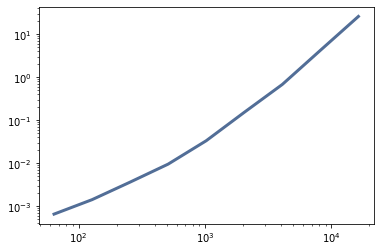
\includegraphics[width=0.75\textwidth]{lab6_fig1_1.png}
        \caption{Визуализация данных с \texttt{analyze1}}
        \label{fig:lab6_fig1_1}
\end{figure}

Наклон близок к 2, а не к 3. Одна из причин состоит в том, что производительность \texttt{np.linalg.solve} почти квадратична в этом диапазоне размеров массива.

Линия изогнута, что говорит нам о том, что мы не достигли размера массива, при котором среда выполнения показывает кубический рост. Я думаю, что при больших размерах массива наклон в конечном итоге сходится к 3.

Теперь рассмотрим результат для \texttt{analyze2}:

\begin{lstlisting}[caption=Работа с \texttt{analyze2}]
results = []
for N in ns:
    ts = (0.5 + np.arange(N)) / N
    freqs = (0.5 + np.arange(N)) / 2
    ys = noise.ys[:N]
    result = %timeit -r1 -o dct.analyze2(ys, freqs, ts)
    results.append(result)

bests2 = [result.best for result in results]
plot_bests(bests2)
\end{lstlisting}

\begin{lstlisting}[caption=Результат работы, literate={µ}{$\upmu$}1 {±}{$\pm$}2]
42.5 µs ± 0 ns per loop (mean ± std. dev. of 1 run, 10000 loops each)
212 µs ± 0 ns per loop (mean ± std. dev. of 1 run, 1000 loops each)
1.04 ms ± 0 ns per loop (mean ± std. dev. of 1 run, 1000 loops each)
3.22 ms ± 0 ns per loop (mean ± std. dev. of 1 run, 100 loops each)
12.2 ms ± 0 ns per loop (mean ± std. dev. of 1 run, 100 loops each)
47.9 ms ± 0 ns per loop (mean ± std. dev. of 1 run, 10 loops each)
189 ms ± 0 ns per loop (mean ± std. dev. of 1 run, 1 loop each)
722 ms ± 0 ns per loop (mean ± std. dev. of 1 run, 1 loop each)
3.05 s ± 0 ns per loop (mean ± std. dev. of 1 run, 1 loop each)

1.9772047966153776
\end{lstlisting}

\begin{figure}[H]
        \centering
        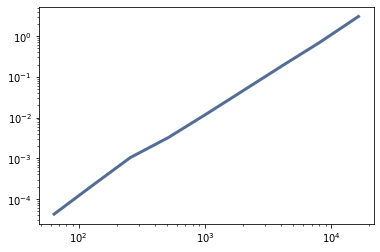
\includegraphics[width=0.75\textwidth]{lab6_fig1_2.png}
        \caption{Визуализация данных с \texttt{analyze2}}
        \label{fig:lab6_fig1_2}
\end{figure}

Результаты для \texttt{analyze2}, как и ожидалось, складываются в прямую линию с предполагаемым наклоном, близким к 2.

Рассмотрим результаты для \texttt{scipy.fftpack.dct}:

\begin{lstlisting}[caption=Работа с \texttt{scipy.fftpack.dct}]
results = []
for N in ns:
    ys = noise.ys[:N]
    result = %timeit -o scipy.fftpack.dct(ys, type=3)
    results.append(result)

bests3 = [result.best for result in results]
plot_bests(bests3)
\end{lstlisting}

\begin{lstlisting}[caption=Результат работы, literate={µ}{$\upmu$}1 {±}{$\pm$}2]
5.33 µs ± 538 ns per loop (mean ± std. dev. of 7 runs, 100000 loops each)
5.25 µs ± 171 ns per loop (mean ± std. dev. of 7 runs, 100000 loops each)
6.55 µs ± 408 ns per loop (mean ± std. dev. of 7 runs, 100000 loops each)
7.7 µs ± 128 ns per loop (mean ± std. dev. of 7 runs, 100000 loops each)
9.5 µs ± 339 ns per loop (mean ± std. dev. of 7 runs, 100000 loops each)
14.9 µs ± 407 ns per loop (mean ± std. dev. of 7 runs, 100000 loops each)
27.3 µs ± 141 ns per loop (mean ± std. dev. of 7 runs, 10000 loops each)
54.5 µs ± 470 ns per loop (mean ± std. dev. of 7 runs, 10000 loops each)
107 µs ± 797 ns per loop (mean ± std. dev. of 7 runs, 10000 loops each)

0.5564395911984347
\end{lstlisting}

\begin{figure}[H]
        \centering
        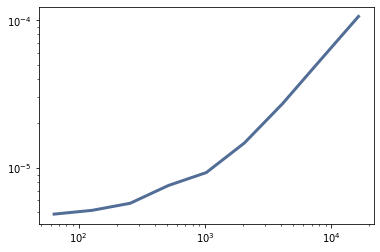
\includegraphics[width=0.75\textwidth]{lab6_fig1_3.png}
        \caption{Визуализация данных с \texttt{scipy.fftpack.dct}}
        \label{fig:lab6_fig1_3}
\end{figure}

Эта реализация \texttt{dct} ещё быстрее. Линия изогнута, что означает, что либо мы ещё не видели асимптотическое поведение, либо асимптотическое поведение не является простым показателем $n$. Фактически, как мы скоро увидим, время выполнения пропорционально $nlogn$.

Теперь рассмотрим все кривые на одних осях:

\begin{lstlisting}[caption=Визуализация всех кривых]
thinkplot.preplot(3)
thinkplot.plot(ns, bests, label='analyze1')
thinkplot.plot(ns, bests2, label='analyze2')
thinkplot.plot(ns, bests3, label='fftpack.dct')
thinkplot.config(xscale='log', yscale='log', legend=True, loc='upper left')
\end{lstlisting}

\begin{figure}[H]
        \centering
        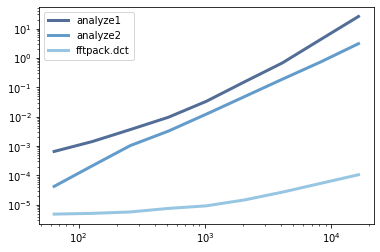
\includegraphics[width=0.75\textwidth]{lab6_fig1_4.png}
        \caption{Визуализация всех кривых}
        \label{fig:lab6_fig1_4}
\end{figure}

\chapter{Упражнение 6.2}

\texttt{thinkdsp} предоставляет класс \texttt{Dct}, похожий на \texttt{Spectrum}, но использующий DCT вместо FFT.

Воспользуемся записью саксофона из предыдущей лабораторной работы:

\begin{lstlisting}[caption=Загрузка звука]
wave = thinkdsp.read_wave('100475__iluppai__saxophone-weep.wav')
wave.make_audio()
\end{lstlisting}

Теперь сделаем короткий сегмент, а затем ДКП этого сегмента:

\begin{lstlisting}[caption=Сегмент звука]
segment = wave.segment(start=2.0, duration=0.5)
segment.normalize()
segment.make_audio()
\end{lstlisting}

\begin{lstlisting}[caption=Сжатие звука]
seg_dct = segment.make_dct()
seg_dct.plot(high=4000)
thinkplot.config(xlabel='Frequency (Hz)', ylabel='DCT')
\end{lstlisting}

\begin{figure}[H]
        \centering
        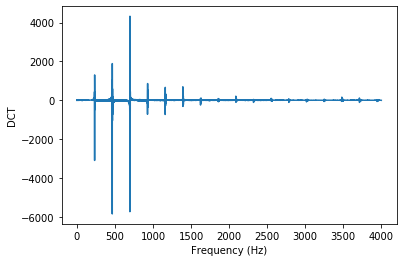
\includegraphics[width=0.75\textwidth]{lab6_fig2_1.png}
        \caption{Визуализация сжатого звука}
        \label{fig:lab6_fig2_1}
\end{figure}

Есть только несколько гармоник со значительной амплитудой, и многие записи близки к нулю. Следующая функция принимает ДКП и устанавливает для элементов ниже порога значение 0.

\begin{lstlisting}[caption=Функция \texttt{compress}]
def compress(dct, thresh=1):
    count = 0
    for i, amp in enumerate(dct.amps):
        if abs(amp) < thresh:
            dct.hs[i] = 0
            count += 1
            
    n = len(dct.amps)
    print(count, n, 100 * count / n, sep='\t')
\end{lstlisting}

Если мы применим его к сегменту, мы можем удалить более 90% элементов:

\begin{lstlisting}[caption=Сжатие звука]
seg_dct = segment.make_dct()
compress(seg_dct, thresh=10)
seg_dct.plot(high=4000)
\end{lstlisting}

\begin{figure}[H]
        \centering
        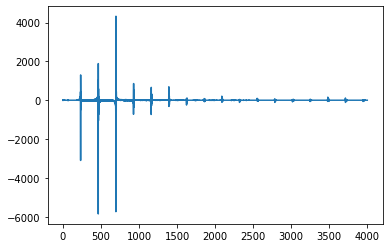
\includegraphics[width=0.75\textwidth]{lab6_fig2_2.png}
        \caption{Визуализация сжатого звука}
        \label{fig:lab6_fig2_2}
\end{figure}

\begin{lstlisting}[caption=Воспроизведение сжатого звука]
seg2 = seg_dct.make_wave()
seg2.make_audio()
\end{lstlisting}

Результат звучит точно так же, по ощущениям ничего не изменилось.

Чтобы сжать более длинный сегмент, мы можем сделать спектрограмму ДКП. Следующая функция похожа на \texttt{wave.make\_spectrogram} за исключением того, что использует ДКП.

\begin{lstlisting}[caption=Функция \texttt{make\_dct\_spectrogram}]
def make_dct_spectrogram(wave, seg_length):
    """Computes the DCT spectrogram of the wave.

    seg_length: number of samples in each segment

    returns: Spectrogram
    """
    window = np.hamming(seg_length)
    i, j = 0, seg_length
    step = seg_length // 2

    # map from time to Spectrum
    spec_map = {}

    while j < len(wave.ys):
        segment = wave.slice(i, j)
        segment.window(window)

        # the nominal time for this segment is the midpoint
        t = (segment.start + segment.end) / 2
        spec_map[t] = segment.make_dct()

        i += step
        j += step

    return thinkdsp.Spectrogram(spec_map, seg_length)
\end{lstlisting}

Теперь мы можем составить DCT-спектрограмму и применить сжатие к каждому сегменту:

\begin{lstlisting}[caption=Сжатие звука]
spectro = make_dct_spectrogram(wave, seg_length=1024)
for t, dct in sorted(spectro.spec_map.items()):
    compress(dct, thresh=0.2)
\end{lstlisting}

В большинстве сегментов сжатие составляет 75-80\%. Чтобы услышать, как это звучит, мы можем преобразовать спектрограмму обратно в волну и воспроизвести её.

\begin{lstlisting}[caption=Воспроизведение сжатого звука]
wave2 = spectro.make_wave()
wave2.make_audio()
\end{lstlisting}

Так же прослушаем оригинал для сравнения.

\begin{lstlisting}[caption=Воспроизведение оригинального звука]
wave.make_audio()
\end{lstlisting}

При сжатии слышно характерный треск во время воспроизведения аудио, так что можно смело сказать, что нам удалось сжать аудиозапись.

\chapter{Упражнение 6.3}
\section{Пилообразная волна}

Для начала воспользуемся пилообразной формой волны, а затем перейдём к более естественным звукам.

\begin{lstlisting}[caption=Создание пилообразного сигнала]
signal = thinkdsp.SawtoothSignal(freq=300, offset=0)
wave = signal.make_wave(duration=0.5, framerate=40000)
wave.make_audio()
\end{lstlisting}

\begin{lstlisting}[caption=Визуализация сигнала]
wave.segment(duration=0.01).plot()
\end{lstlisting}

\begin{figure}[H]
        \centering
        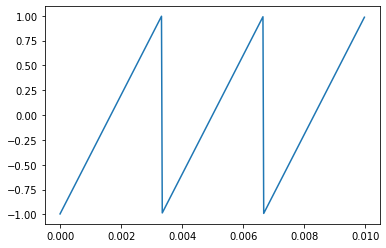
\includegraphics[width=0.75\textwidth]{lab6_fig3_1.png}
        \caption{Визуализация сигнала}
        \label{fig:lab6_fig3_1}
\end{figure}

\begin{lstlisting}[caption=Спектр сигнала]
spectrum = wave.make_spectrum()
spectrum.plot()
\end{lstlisting}

\begin{figure}[H]
        \centering
        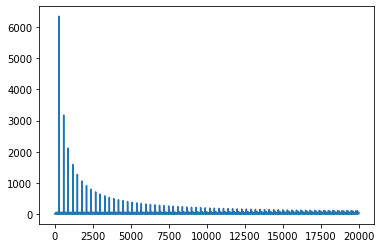
\includegraphics[width=0.75\textwidth]{lab6_fig3_2.png}
        \caption{Спектр сигнала}
        \label{fig:lab6_fig3_2}
\end{figure}

Рассмотрим угловую часть спектра при помощи функции \texttt{plot\_angle}.

\begin{lstlisting}[caption=Функция \texttt{plot\_angle}]
def plot_angle(spectrum, thresh=1):
    angles = spectrum.angles
    angles[spectrum.amps < thresh] = np.nan
    thinkplot.plot(spectrum.fs, angles, style='x')
    thinkplot.config(xlim=[0, spectrum.max_freq],
                     ylim =[-np.pi, np.pi])
\end{lstlisting}

На большинстве частот амплитуда мала, а угол - в значительной степени случайное число. Так что если мы построим все углы, получится небольшой беспорядок.

\begin{lstlisting}[caption=Визуализация угловой части спектра с tresh = 0]
plot_angle(spectrum, thresh=0)
thinkplot.config(xlim=[0, spectrum.max_freq], ylim = [-np.pi, np.pi])
\end{lstlisting}

\begin{figure}[H]
        \centering
        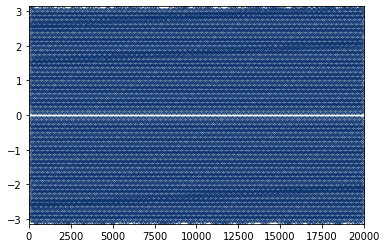
\includegraphics[width=0.75\textwidth]{lab6_fig3_3.png}
        \caption{Визуализация угловой части спектра с tresh = 0}
        \label{fig:lab6_fig3_3}
\end{figure}

\begin{lstlisting}[caption=Визуализация угловой части спектра с tresh = 1]
plot_angle(spectrum, thresh=1)
thinkplot.config(xlim=[0, spectrum.max_freq], ylim = [-np.pi, np.pi])
\end{lstlisting}

\begin{figure}[H]
        \centering
        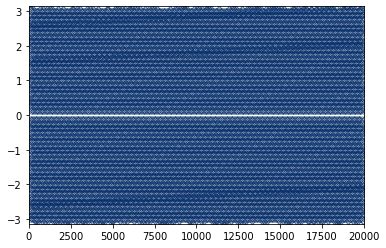
\includegraphics[width=0.75\textwidth]{lab6_fig3_4.png}
        \caption{Визуализация угловой части спектра с tresh = 1}
        \label{fig:lab6_fig3_4}
\end{figure}

Когда мы выбираем только те частоты, где величина превышает пороговое значение, мы видим, что в углах есть структура. Каждая гармоника смещена от предыдущей на доли радиана.

Следующая функция отображает амплитуды, углы и форму волны для заданного спектра.

\begin{lstlisting}[caption=Функция \texttt{plot\_three}]
def plot_three(spectrum, thresh=1):
    thinkplot.preplot(cols=3)
    spectrum.plot()
    thinkplot.subplot(2)
    plot_angle(spectrum, thresh=thresh)
    thinkplot.subplot(3)
    wave = spectrum.make_wave()
    wave.segment(duration=0.01).plot()
    wave.apodize()
    display(wave.make_audio())
\end{lstlisting}

Теперь мы можем визуализировать неизменённый спектр:

\begin{lstlisting}[caption=Визуализация неизменённого спектра]
plot_three(spectrum)
\end{lstlisting}

\begin{figure}[H]
        \centering
        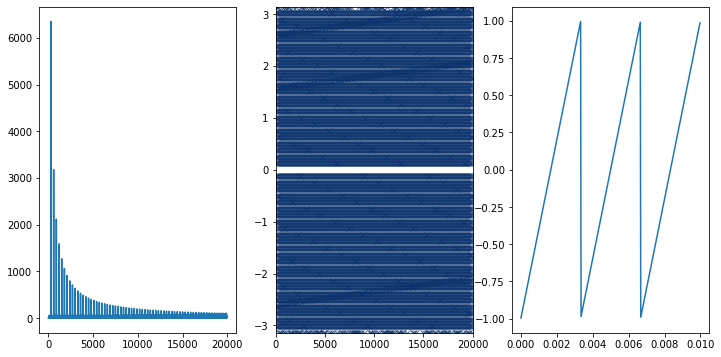
\includegraphics[width=0.75\textwidth]{lab6_fig3_5.png}
        \caption{Визуализация неизменённого спектра}
        \label{fig:lab6_fig3_5}
\end{figure}

Теперь рассмотрим, что произойдёт, если мы установим все углы в ноль.

\begin{lstlisting}[caption=Функция \texttt{zero\_angle}]
def zero_angle(spectrum):
    res = spectrum.copy()
    res.hs = res.amps
    return res
\end{lstlisting}

Амплитуды не изменились, все углы равны нулю, и форма волны выглядит совсем иначе. Но волна звучит примерно так же, только появился какой-то шум, да и громкость стала немного ниже.

\begin{lstlisting}[caption=Визуализация при нулевых углах]
spectrum2 = zero_angle(spectrum)
plot_three(spectrum2)
\end{lstlisting}

\begin{figure}[H]
        \centering
        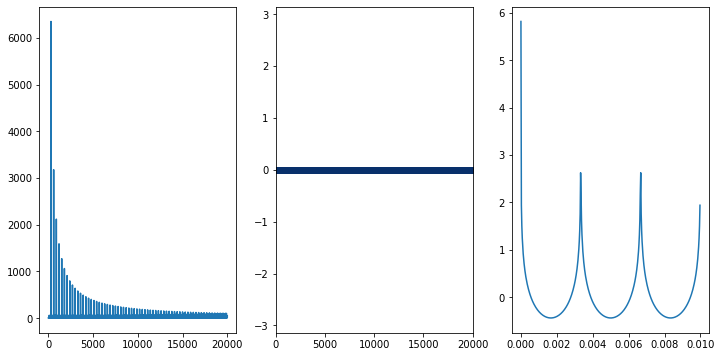
\includegraphics[width=0.75\textwidth]{lab6_fig3_6.png}
        \caption{Визуализация при нулевых углах}
        \label{fig:lab6_fig3_6}
\end{figure}

Если мы умножим комплексные компоненты на $exp(i\phi)$ это приведет к добавлению $\phi$ к углам:

\begin{lstlisting}[caption=Функция \texttt{rotate\_angle}]
def rotate_angle(spectrum, offset):
    res = spectrum.copy()
    res.hs *= np.exp(1j * offset)
    return res
\end{lstlisting}

Эффект можно увидеть на рисунке ниже. Опять же, форма волны другая, но звучит примерно так же.

\begin{lstlisting}[caption=Визуализация при повороте углов]
spectrum3 = rotate_angle(spectrum, 1)
plot_three(spectrum3)
\end{lstlisting}

\begin{figure}[H]
        \centering
        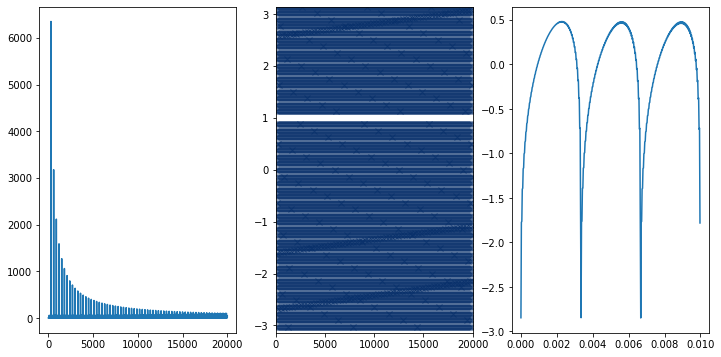
\includegraphics[width=0.75\textwidth]{lab6_fig3_7.png}
        \caption{Визуализация при повороте углов}
        \label{fig:lab6_fig3_7}
\end{figure}

Теперь рассмотрим случай, если мы установим углы на случайные значения.

\begin{lstlisting}[caption=Функция \texttt{random\_angle}]
PI2 = np.pi * 2

def random_angle(spectrum):
    res = spectrum.copy()
    angles = np.random.uniform(0, PI2, len(spectrum))
    res.hs *= np.exp(1j * angles)
    return res
\end{lstlisting}

Влияние на форму волны сильное, но воспринимаемый звук остаётся плюс минус прежним, правда он приобрёл "металлический" эффект.

\begin{lstlisting}[caption=Визуализация при случайных углах]
spectrum4 = random_angle(spectrum)
plot_three(spectrum4)
\end{lstlisting}

\begin{figure}[H]
        \centering
        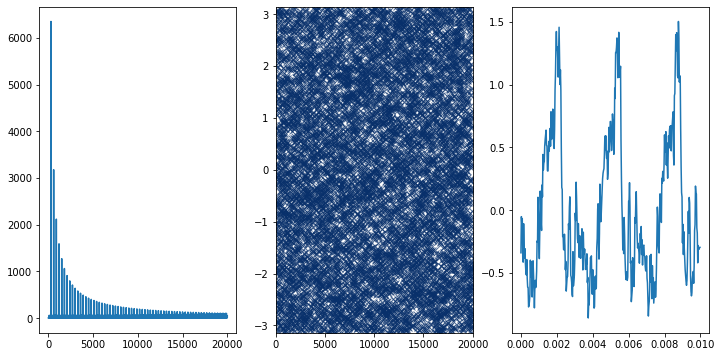
\includegraphics[width=0.75\textwidth]{lab6_fig3_8.png}
        \caption{Визуализация при случайных углах}
        \label{fig:lab6_fig3_8}
\end{figure}

\section{Запись габоя}

С более естественными звуками результаты несколько отличаются. Рассмотрим запись гобоя.

\begin{lstlisting}[caption=Загрузка звука]
wave = thinkdsp.read_wave('120994__thirsk__120-oboe.wav')
wave.make_audio()
\end{lstlisting}

\begin{lstlisting}[caption=Визуализация неизменённого звука]
segment = wave.segment(start=0.2, duration=0.6)
spectrum = segment.make_spectrum()
plot_three(spectrum, thresh=50)
\end{lstlisting}

\begin{figure}[H]
        \centering
        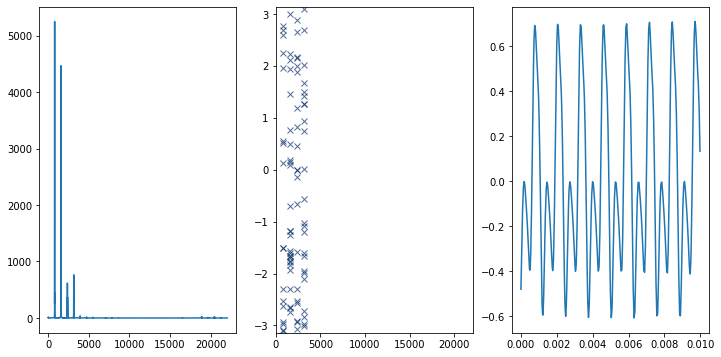
\includegraphics[width=0.75\textwidth]{lab6_fig3_9.png}
        \caption{Визуализация неизменённого звука}
        \label{fig:lab6_fig3_9}
\end{figure}

Здесь все углы установлены в ноль.

\begin{lstlisting}[caption=Визуализация при нулевых углах]
spectrum2 = zero_angle(spectrum)
plot_three(spectrum2, thresh=50)
\end{lstlisting}

\begin{figure}[H]
        \centering
        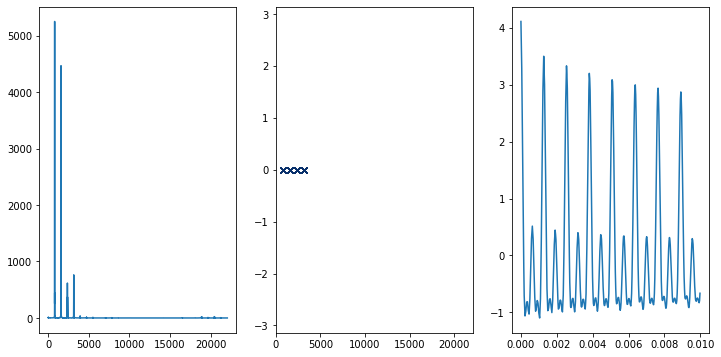
\includegraphics[width=0.75\textwidth]{lab6_fig3_10.png}
        \caption{Визуализация при нулевых углах}
        \label{fig:lab6_fig3_10}
\end{figure}

Теперь рассмотрим случай, когда углы повёрнуты на 1 радиан.

\begin{lstlisting}[caption=Визуализация при повороте углов]
spectrum3 = rotate_angle(spectrum, 1)
plot_three(spectrum3, thresh=50)
\end{lstlisting}

\begin{figure}[H]
        \centering
        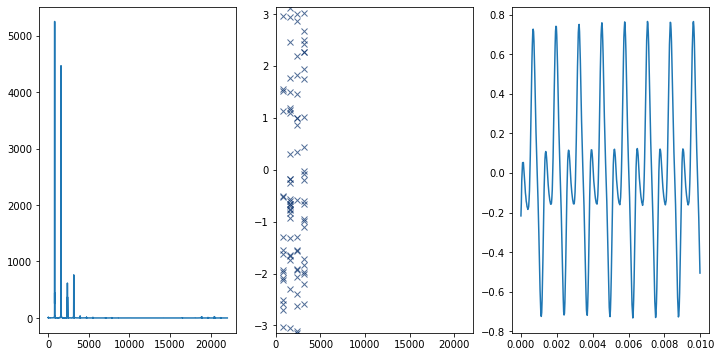
\includegraphics[width=0.75\textwidth]{lab6_fig3_11.png}
        \caption{Визуализация при повороте углов}
        \label{fig:lab6_fig3_11}
\end{figure}

Теперь рассмотрим случайные углы.

\begin{lstlisting}[caption=Визуализация при случайных углах]
spectrum4 = random_angle(spectrum)
plot_three(spectrum4, thresh=50)
\end{lstlisting}

\begin{figure}[H]
        \centering
        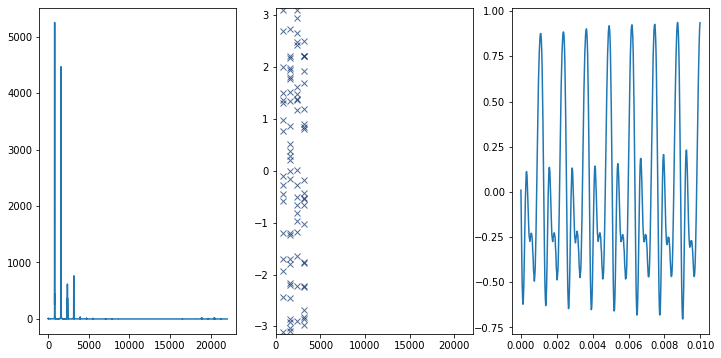
\includegraphics[width=0.75\textwidth]{lab6_fig3_12.png}
        \caption{Визуализация при случайных углах}
        \label{fig:lab6_fig3_12}
\end{figure}

Как мне кажется, установка углов в ноль снижает громкость, поворот углов не имеет вообще никакого эффекта, а случайные углы придают звуку какой-то эффект реверберации.

Попробуем то же самое с отрывком из записи саксофона.

\section{Запись саксофона}

\begin{lstlisting}[caption=Загрузка звука]
wave = thinkdsp.read_wave('100475__iluppai__saxophone-weep.wav')
wave.make_audio()
\end{lstlisting}

\begin{lstlisting}[caption=Визуализация неизменённого звука]
segment = wave.segment(start=2.5, duration=0.6)
spectrum = segment.make_spectrum()
plot_three(spectrum, thresh=50)
\end{lstlisting}

\begin{figure}[H]
        \centering
        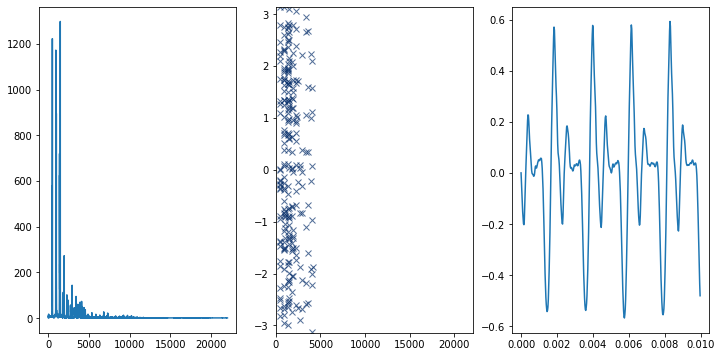
\includegraphics[width=0.75\textwidth]{lab6_fig3_13.png}
        \caption{Визуализация неизменённого звука}
        \label{fig:lab6_fig3_13}
\end{figure}

Здесь все углы установлены в ноль.

\begin{lstlisting}[caption=Визуализация при нулевых углах]
spectrum2 = zero_angle(spectrum)
plot_three(spectrum2, thresh=50)
\end{lstlisting}

\begin{figure}[H]
        \centering
        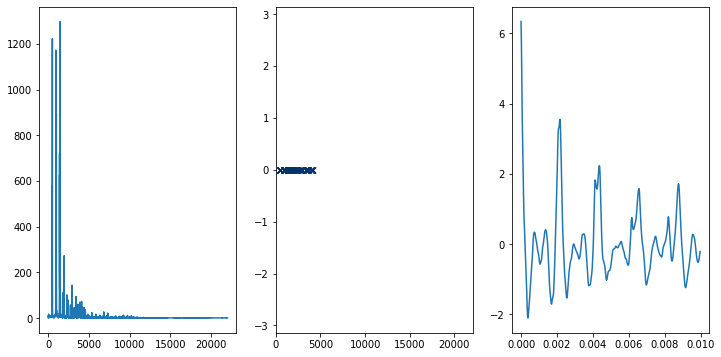
\includegraphics[width=0.75\textwidth]{lab6_fig3_14.png}
        \caption{Визуализация при нулевых углах}
        \label{fig:lab6_fig3_14}
\end{figure}

Теперь рассмотрим случай, когда углы повёрнуты на 1 радиан.

\begin{lstlisting}[caption=Визуализация при повороте углов]
spectrum3 = rotate_angle(spectrum, 1)
plot_three(spectrum3, thresh=50)
\end{lstlisting}

\begin{figure}[H]
        \centering
        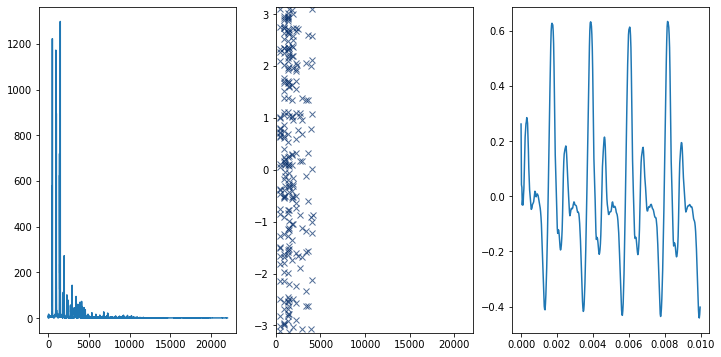
\includegraphics[width=0.75\textwidth]{lab6_fig3_15.png}
        \caption{Визуализация при повороте углов}
        \label{fig:lab6_fig3_15}
\end{figure}

Теперь рассмотрим случайные углы.

\begin{lstlisting}[caption=Визуализация при случайных углах]
spectrum4 = random_angle(spectrum)
plot_three(spectrum4, thresh=50)
\end{lstlisting}

\begin{figure}[H]
        \centering
        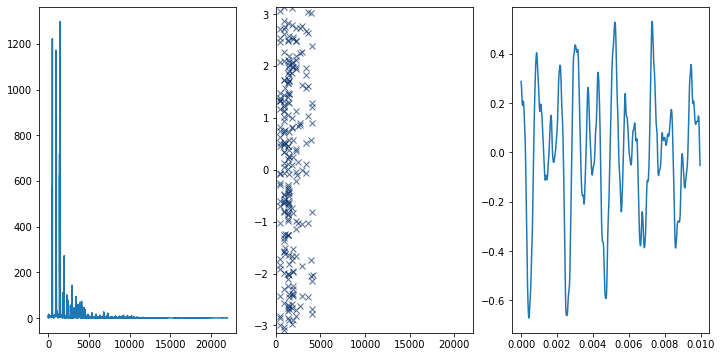
\includegraphics[width=0.75\textwidth]{lab6_fig3_16.png}
        \caption{Визуализация при случайных углах}
        \label{fig:lab6_fig3_16}
\end{figure}

Прослушав все звуки можно сделать вывод, что обнуление делает со звуком какие-то странные вещи, будто бы он стал каким-то "пьяным", вращение вновь не имеет никакого эффекта, а случайные углы добавляют вновь эффект реверберации.

Также я знаю, что саксофон отличается от других звуков тем, что основной компонент не является доминирующим. Я предполагаю, что для подобных звуков ухо использует что-то вроде автокорреляции в дополнение к спектральному анализу, и возможно, что этот вторичный режим анализа более чувствителен к фазовой структуре.

Если это так, эффект должен быть более сильным, если фундаментальный вообще отсутствует. Давайте в этом убедимся.

\section{Урезание фундаментальных гармоник}

\begin{lstlisting}[caption=Урезание частот звука]
spectrum.high_pass(600)
spectrum.plot(high=4000)
\end{lstlisting}

\begin{figure}[H]
        \centering
        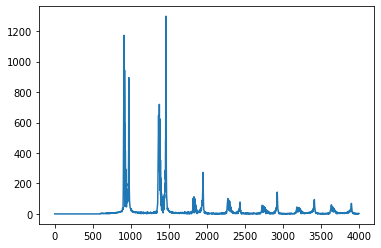
\includegraphics[width=0.75\textwidth]{lab6_fig3_17.png}
        \caption{Урезание частот звука}
        \label{fig:lab6_fig3_17}
\end{figure}

\begin{lstlisting}[caption=Визуализация неизменённого звука]
segment = wave.segment(start=2.5, duration=0.6)
spectrum = segment.make_spectrum()
plot_three(spectrum, thresh=50)
\end{lstlisting}

\begin{figure}[H]
        \centering
        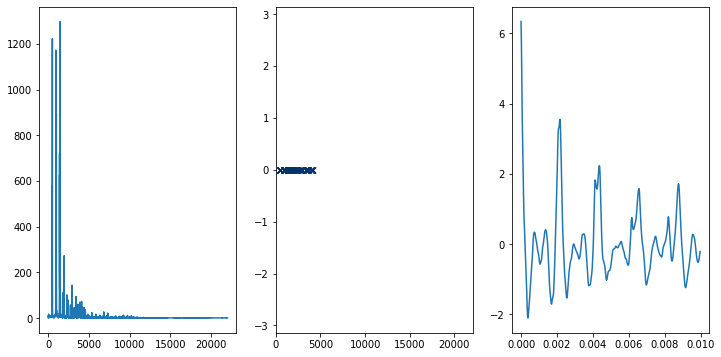
\includegraphics[width=0.75\textwidth]{lab6_fig3_18.png}
        \caption{Визуализация неизменённого звука}
        \label{fig:lab6_fig3_18}
\end{figure}

Здесь все углы установлены в ноль.

\begin{lstlisting}[caption=Визуализация при нулевых углах]
spectrum2 = zero_angle(spectrum)
plot_three(spectrum2, thresh=50)
\end{lstlisting}

\begin{figure}[H]
        \centering
        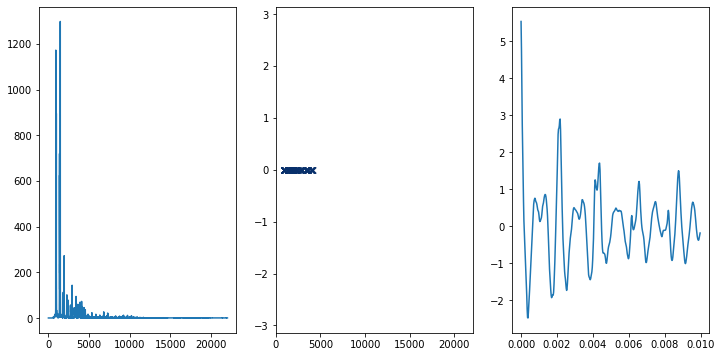
\includegraphics[width=0.75\textwidth]{lab6_fig3_19.png}
        \caption{Визуализация при нулевых углах}
        \label{fig:lab6_fig3_19}
\end{figure}

Теперь рассмотрим случай, когда углы повёрнуты на 1 радиан.

\begin{lstlisting}[caption=Визуализация при повороте углов]
spectrum3 = rotate_angle(spectrum, 1)
plot_three(spectrum3, thresh=50)
\end{lstlisting}

\begin{figure}[H]
        \centering
        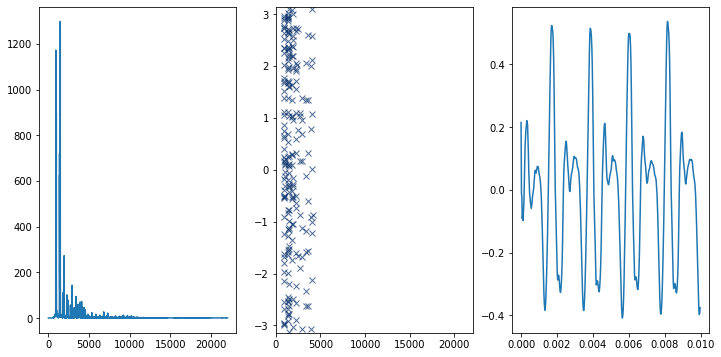
\includegraphics[width=0.75\textwidth]{lab6_fig3_20.png}
        \caption{Визуализация при повороте углов}
        \label{fig:lab6_fig3_20}
\end{figure}

Теперь рассмотрим случайные углы.

\begin{lstlisting}[caption=Визуализация при случайных углах]
spectrum4 = random_angle(spectrum)
plot_three(spectrum4, thresh=50)
\end{lstlisting}

\begin{figure}[H]
        \centering
        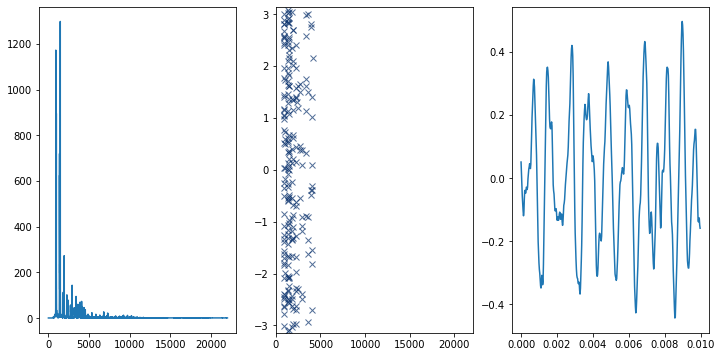
\includegraphics[width=0.75\textwidth]{lab6_fig3_21.png}
        \caption{Визуализация при случайных углах}
        \label{fig:lab6_fig3_21}
\end{figure}

Для этого сегмента изменение фазовой структуры имеет слышимый эффект, особенно случайные углы.

Если ухо использует что-то вроде автокорреляции для анализа подобных звуков, мы можем ожидать увидеть изменения в функции автокорреляции при изменении фазовой структуры.

\section{Построение АКФ}

Следующие функции строят АКФ для этих сегментов:

\begin{lstlisting}[caption=Функция \texttt{autocorr}]
def autocorr(segment):
    corrs = np.correlate(segment.ys, segment.ys, mode='same')
    N = len(corrs)
    lengths = range(N, N//2, -1)

    half = corrs[N//2:].copy()
    half /= lengths
    half /= half[0]
    return half
\end{lstlisting}

\begin{lstlisting}[caption=Функция \texttt{plot\_acf}]
def plot_acf(spectrum):
    corrs = autocorr(spectrum.make_wave())
    thinkplot.plot(corrs[:200], linewidth=1)
\end{lstlisting}

\begin{lstlisting}[caption=Построение АКФ]
plot_acf(spectrum)
plot_acf(spectrum2)
plot_acf(spectrum3)
plot_acf(spectrum4)
thinkplot.config(xlabel='Lag', ylabel='Correlation', ylim=[-1.05, 1.05])
\end{lstlisting}

\begin{figure}[H]
        \centering
        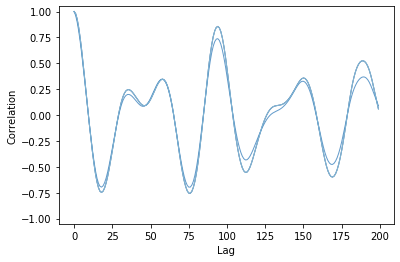
\includegraphics[width=0.75\textwidth]{lab6_fig3_22.png}
        \caption{Построение АКФ}
        \label{fig:lab6_fig3_22}
\end{figure}

Как мне кажется, изменение фазовой структуры оказывает некоторое влияние на АКФ, но не так сильно, и там нет ничего, что явно объясняет изменения в воспринимаемом звуке.

По крайней мере, для таких звуков, которые имеют простую гармоническую структуру, мы не слышим изменений в фазовой структуре, при условии, что гармоническая структура не изменилась.

Возможное исключение - звуки с низкой амплитудой на основной частоте. В этом случае мы используем что-то вроде автокорреляции для восприятия высоты звука, и это намек на то, что этот анализ может быть более чувствительным к фазовой структуре. Однако в АКФ нет ничего очевидного, объясняющего этот эффект.

\chapter{Выводы}

Во время выполнения лабораторной работы получены навыки работы с прямым и обратным дискретным косинусным преобразованием. Также получены навыки их практического применения.

\end{document}